\noindent \textbf{Initial Sizing Report}\\
\textbf{Group 19}

\section{Group scenario}
Location and climate type: Leeuwarden, Netherlands (cold)\\
Number of households and load profile: 50(A) \\
Primary source of energy: Wind \\
Secondary source of energy: Biomass \\
Battery type: Vanadium redox flow \\ 


\section{Location and motivation}

The location chosen for our project is Leeuwarden, Netherlands. The wind climate characteristics of the Leeuwarden, and its close proximity to the sea, indicates potential sites for wind turbines, and farms \citep{Power}. Thus, Wind Energy is a suitable primary source. Also, since there are number of farmlands in Leeuwarden, the choice for secondary source is Biomass.

\section{Per-second randomized load curve for 2 min}
\begin{figure} [H]
    \centering
    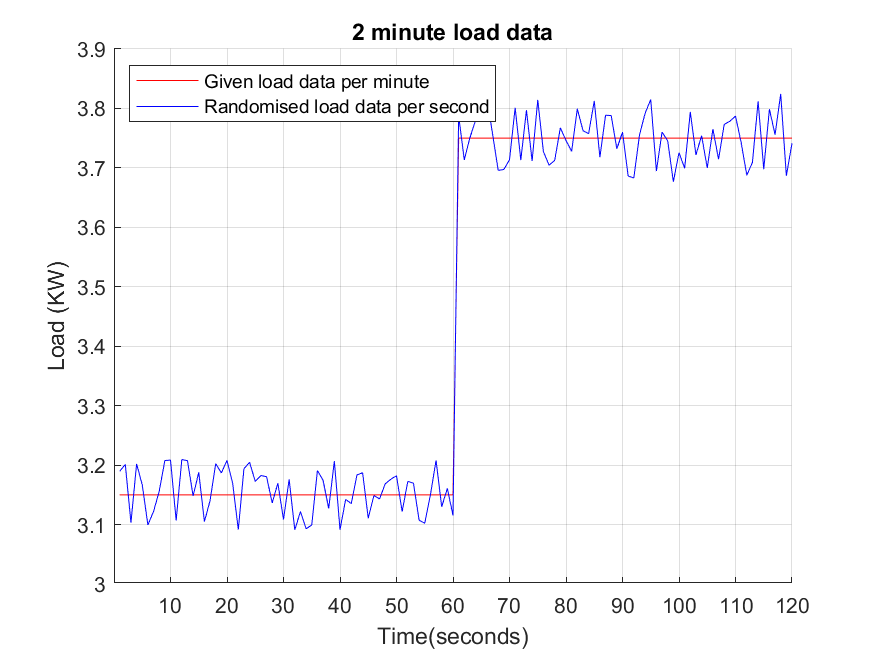
\includegraphics[width=0.5 \linewidth]{w1/images/two_min_load_comparison.png}
    \caption{2 minute load comparison after randomization}
    \label{fig:2_min_load}
\end{figure}

\section{Plot for week}
\begin{figure} [H]
    \centering
    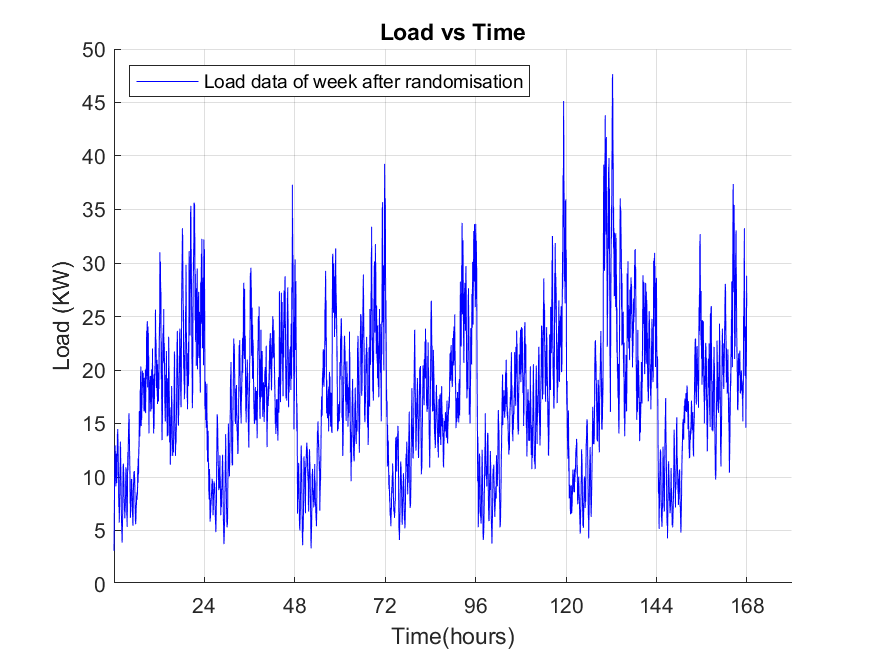
\includegraphics[width=0.5 \linewidth]{w1/images/Load_after_randomization.png}
    \caption{Load data for week after randomization}
    \label{fig:load_for_week}
\end{figure}

\section{Primary, secondary, and battery type}


\subsection{Logic behind initial sizing}
The main logic involved considering the cost and zero exchange constraints is that the average load should always be catered by the primary source. Since we have wind power as the primary source, the type of turbine chosen is such that it caters to the average load at average wind speed. Therefore, the peak load should be catered by the combination of primary and secondary sources ( around 60\% by primary and 40\% by secondary).   
Batteries are used to compensate the load during the cold start-up time of CHP plant. Hence the sizing of batteries is done as follows:
 \begin{equation}
    Required\quad battery\quad energy\quad  density = \frac{Lag\quad time\quad X\quad Load\quad to\quad be\quad compensated}{Conversion\quad Efficiency} 
 \end{equation}
 where,  Load to be compensated = secondary source capacity


\subsection{Type of wind turbine (primary source)}

From the site wind data, the average wind speed at 10m height was determined to be 5.1 m/s. The wind turbine chosen for this location is the Vestas V25: 200KW. This model was chosen instead of other similar models, due to its proven track record indicating higher reliability, and lower cut-in speed (thereby utilizing lower values in wind distribution).\\ 
Vestas V25: 200KW\\
$V_{cut-in}$ = 3.5 m/s\\
$V_{rated}$ = 11.5 m/s\\
$V_{cut-out}$ = 25 m/s\\
Output voltage = 480 V
Diameter = 25m\\
Hub height = 35 m\\
Power at average wind speed = 25KW




\subsection{Sizing}

Micro-grid voltage = 230V \\
\textbf{Primary source sizing:}\\
Turbine rating = 200kW\\
Number of turbines = 1\\
\textbf{Secondary source sizing:}\\
Biomass (CHP) plant rating = 74kW \\
Biogas-to-Electricity efficiency: 30$\%$ \\
\textbf{Battery sizing:}\\
Battery type: Vanadium Redox flow batteries were chosen as they are cheap and are commercially used for grid stability. \\
Battery Voltage: 1.4V\\
Capacity: 26.8Ah\\
Efficiency: 76$\%$ \\
Number of batteries = 155\\
Amount of electrolyte required: 170 litre\\
SOC max = 80$\%$\\
SOC min= 20$\%$


\section{Summary}

\begin{table}[H]
\begin{tabular}{|l|l|l|l|l|l|}
\hline
\textbf{Parameters}   & \textbf{Average load}  & \textbf{Peak load}     & \textbf{Primary source} & \textbf{Secondary source} & \textbf{Batteries}                                                                                                          \\ \hline
\multirow{2}{*}{Size} & \multirow{2}{*}{17 KW} & \multirow{2}{*}{47 KW} & \multirow{2}{*}{200 KW} & \multirow{2}{*}{74 KW}    & \multirow{2}{*}{\begin{tabular}[c]{@{}l@{}}155 VRF batteries(1.4V, 26.8Ah)\\ SOC: 20$\%$(min) to 80$\%$(max)\end{tabular}} \\
                      &                        &                        &                         &                           &                                                                                                                             \\ \hline
\end{tabular}
\end{table}



